\documentclass[12pt]{article}
\setlength\parindent{0pt}
\usepackage{fullpage}
\usepackage{amsmath}
\usepackage{graphicx}
\usepackage{color}
\definecolor{Red}           {rgb}{1,0.3,0.0}
\setlength{\parskip}{4mm}
\def\LL{\left\langle}   % left angle bracket
\def\RR{\right\rangle}  % right angle bracket
\def\LP{\left(}         % left parenthesis
\def\RP{\right)}        % right parenthesis
\def\LB{\left\{}        % left curly bracket
\def\RB{\right\}}       % right curly bracket
\def\PAR#1#2{ {{\partial #1}\over{\partial #2}} }
\def\PARTWO#1#2{ {{\partial^2 #1}\over{\partial #2}^2} }
\def\PARTWOMIX#1#2#3{ {{\partial^2 #1}\over{\partial #2 \partial #3}} }
\newcommand{\BI}{\begin{itemize}}
\newcommand{\EI}{\end{itemize}}
\newcommand{\BE}{\begin{displaymath}}
\newcommand{\EE}{\end{displaymath}}
\newcommand{\BNE}{\begin{equation}}
\newcommand{\ENE}{\end{equation}}
\newcommand{\BEA}{\begin{eqnarray}}
\newcommand{\EEA}{\nonumber\end{eqnarray}}
\newcommand{\EL}{\nonumber\\}
\newcommand{\la}[1]{\label{#1}}
\newcommand{\ie}{{\em i.e.\ }}
\newcommand{\eg}{{\em e.\,g.\ }}
\newcommand{\cf}{cf.\ }
\newcommand{\etc}{etc.\ }
\newcommand{\Tr}{{\rm tr}}
\newcommand{\etal}{{\it et al.}}
\newcommand{\OL}[1]{\overline{#1}\ } % overline
\newcommand{\OLL}[1]{\overline{\overline{#1}}\ } % double overline
\newcommand{\OON}{\frac{1}{N}} % "one over N"
\newcommand{\OOX}[1]{\frac{1}{#1}} % "one over X"



\begin{document}
\pagenumbering{gobble}
\Large
\centerline{\sc{Recitation Exercises}}
\normalsize
\centerline{\{(This didn't get printed with the main set because of a mixup, sorry!)}

\medskip
\centerline{\Large Question 1: Practice from Earlier (this should be quick)}

\begin{minipage}{0.5\textwidth}
	Consider a ball tethered to a rotating pole by two cables of equal length as shown to the right. The ball rotates along with the pole, making a horizontal circle (shown in green on the diagram). Suppose that you know the ball has a mass $m$, the pole is rotating at angular velocity $\omega$, and the radius of the circle it makes is $r$.
	
	\bigskip
	
	You want to find the relationship between $m$, $\omega$, $r$, and the tensions in the cables $T_1$ and $T_2$.
	
\end{minipage}
\begin{minipage}{0.4\textwidth}
	\hspace{0.1\textwidth}
	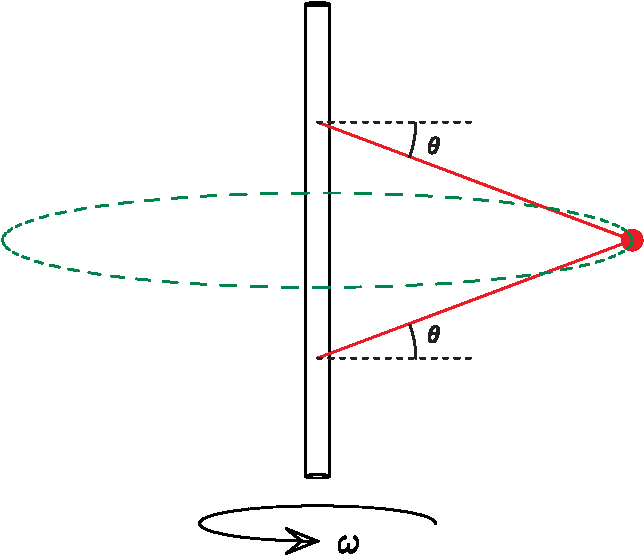
\includegraphics[width=0.9\textwidth]{pole-crop.pdf}
\end{minipage}

Draw a force diagram for the ball below, and indicate your choice of coordinate system.
%
%{\color{Red} This is just for practice in case anyone gets done or wants extra practice. This is a former exam problem.}

\vspace{3in}

Construct Newton's laws in both $x$ and $y$ for the ball based on your force diagram, putting in what you know about $a_x$ and $a_y$. (You don't need to actually solve the system of equations, but show it to your TA/coach.)
%
%{\color{Red}
%
%\begin{align*}
%T_1 \cos \theta + T_2 \cos \theta\hspace{2.6em} &= m \omega^2 r \\
%T_1 \sin \theta - T_2 \sin \theta - mg &= 0
%\end{align*}
%
%They shouldn't feel the need to go any further than this.



\end{document}
